\documentclass[aps,pre,
superscriptaddress,
twocolumn,
notitlepage,
10pt,
]{revtex4-1}

%              longbibliography,


\usepackage[utf8]{inputenc}
% \usepackage{inputenc}[latin9] 
\usepackage[T1]{fontenc}
\usepackage{amsmath, amssymb, amsfonts, bm}
\usepackage{graphicx}
\usepackage{color}
\usepackage{float}
\usepackage[%
colorlinks=true,
urlcolor=black,
linkcolor=blue,
citecolor=blue
]{hyperref}


%\usepackage{dcolumn}
\usepackage{subfigure} 


\hyphenation{Figure}

\setlength{\textfloatsep}{10pt plus 1.0pt minus 2.0pt}


\begin{document} 

\title{Flow through Self-Affine Fractures}

\author{H. J. Seybold} %\email{hseybold@ethz.ch}
\affiliation{Physics of Environmental Systems, D-USYS, ETH, Zurich, 8093
	Zurich, Switzerland}

\author{H. A. Carmona} %\email{carmona@fisica.ufc.br}
\affiliation{Departamento de F\'isica, Universidade Federal do Cear\'a,
	Campus do Pici, 60451-970 Fortaleza, Cear\'a, Brazil}

\author{F. A. Leandro Filho} %\email{leandro.filho@fisica.ufc.br}
\affiliation{Departamento de F\'isica, Universidade Federal do Cear\'a,
	Campus do Pici, 60451-970 Fortaleza, Cear\'a, Brazil}



% \author{Alex Hansen} %\email{alex.hansen@ntnu.no}
% \affiliation{Department of Physics, Norwegian University of Science and
% Technology, N?7491 Trondheim, Norway}

\author{A. D. Ara\'ujo} %\email{ascanio@fisica.ufc.br}
\affiliation{Departamento de F\'isica, Universidade Federal do Cear\'a,
	Campus do Pici, 60451-970 Fortaleza, Cear\'a, Brazil}

\author{F. Nepomuceno Filho}
\affiliation{Departamento de F\'isica, Universidade Federal do Cear\'a,
	Campus do Pici, 60451-970 Fortaleza, Cear\'a, Brazil}

\author{J. S. Andrade Jr.} \email{soares@fisica.ufc.br}
\affiliation{Departamento de F\'isica, Universidade Federal do Cear\'a,
	Campus do Pici, 60451-970 Fortaleza, Cear\'a, Brazil}

\begin{abstract} 
	Surface roughness has a considerable influence on the flow resistance of fluids
passing through fracture joints. Using the Hurst exponent $H$ to characterize
the roughness of a self-affine surface, we investigate the impact of inertia on
the flow's resistance as a function of roughness and Reynolds number. We find
that the hydraulic resistance $G\equiv -\Delta P w^{2}/\mu U L$ follows a
universal behavior when the characteristic length scale of the system is
defined by the tortuosity of the surface times the opening of the fracture.
Moreover, we show that the nonlinear corrections to Darcy's law are
proportional to the Hurst exponent at the transition from Stokes to inertial
flow. This result implies that the second and third order corrections to
Darcy's law depend  depend on the permeability even for very rough surfaces ($H
\sim 0.3$). The effective permeability of the fracture decays exponentially
with $H^{-1}$. Our results also reveal the presence of quasi-one-dimensional
channeling of the flow, even when there is no shear displacement between the
upper and lower surfaces constituting the self-affine fracture joints.
\end{abstract}


\maketitle

% Introduction ---------------------------------------------------
\section{Introduction}


Understanding the detailed behavior of a fluid flowing through a fractured rock,
in particular in what way the morphology of the fracture's surfaces influences
the flow resistance is of great importance in many practical
applications~\cite{Sahimi1993, Berkowitz2002, Sahimi2011, Osborn2011,
	Williams2017}.

Fractures have crucial role in driving fluids through naturally fractured
carbonate reservoirs~\cite{Warren1963, Liu2016a}, and hydraulic fracturing
\cite{HUBBERT1957, Rubinstein2015} is a procedure frequently used for oil
recovery. Since at the reservoir scale fractures are mostly composed of networks
of interconnected cracks with very different sizes, it is relevant to understand
how the behavior of the flow in a single fracture scales with its size, as well
as how it is affected by the surface morphology~\cite{Liu2016a}. The local flow
structures are a direct result of the fracture's morphology and many studies
have been dedicated to understand their upscale in order to derive macroscopic
relations~\cite{Roux1993, Talon2010, Talon2010a, Wang2016}.


It has become increasingly clear that the morphology of brittle fractures
follows \emph{self-affine} scaling laws~\cite{Bunde1996}. More precisely, it
means that by re-scaling an in-plane vector $\mathbf{r}$ by $\lambda
\mathbf{r}$, the out-of-plane coordinate $z$ needs to be re-scaled by
$\lambda^{H} z$ for the surface to remain statistically invariant, where the
scaling exponent $H$ is called the Hurst exponent. 
%
It was first suggested that rock fractures have a unique exponent
$H=0.8$~\cite{Bouchaud1990, Maaloey1992, Schmittbuhl1993,
	Cox1993,Schmittbuhl1995,Bouchaud1997, Oron1998}. However, recent evidence
indicates that other values of $H$ also occur in natural systems (ranging from
$0.45$ to $0.85$) depending  on the material and how the fracture has been
produced~\cite{Odling1994,Amitrano2002, Ponson2006, Babadagli2015}. As a result,
more than one universality class exists for fractured rocks and therefore it is
important to understand how the flow properties are affected by variations in
the Hurst exponent.

A single-phase flow in a fractured rock is usually characterized in terms of
Darcy's law~\cite{Sahimi1994,Sahimi2011, Dullien1992}, which defines a linear
relation between the mean flow velocity $ U $ and the pressure drop $\Delta P$
across the system, namely $U = -k \Delta P/\mu L$. Here $\mu$ is the fluid's
viscosity,  $L$ is the length of the fracture in the flow direction, and the
proportionally constant $k$ is the permeability. Essentially Darcy's law is a
good approximation at low Reynolds numbers,
%
$\mathrm{Re} = \rho U w/\mu \ll 1$, 
%
where $w$ is usually taken as the aperture of the fracture and $\rho$ is the
density of the fluid. However, in order to understand the interplay between the
surface's roughness and the flow inside the fracture, it is necessary to examine
\emph{local} aspects of the surface roughness and relate them to the relevant
mechanisms of momentum transfer through viscous and inertial forces.

The influence of surface roughness on the flow properties inside a fracture
has been first studied theoretically by Roux \emph{et al.}~\cite{Roux1993}.
They predicted that the permeability of a self-affine fracture should scale
with the length of the system as $k \sim L^{2H}$. This result is based on
the assumption that the fracture behaves like a system of parallel plates
with an effective aperture $w$, given that self-affinity implies that $w
\sim L^H$, and $k \sim w^2$ follows the solution of the Stokes equation. 

Since then, several theoretical and experimental studies, all focused on
how the permeability scales with the fracture opening and length in the
viscous flow regime, treating it as an equivalent system of parallel
plates. Using perturbation theory, Drazer and Koplik~\cite{Drazer2000}
calculated that the permeability should scale as $k_0 - k \sim L^H$ for
two-dimensional flows, where $k_0$ is the permeability of the unperturbed
system. Later they extended their study to three-dimensional flows and
confirmed their results in terms of the effective medium analysis with
numerical simulations at low Reynolds numbers.
%
Talon \emph{et al.}~\cite{Talon2010} conjectured that the permeability is
controlled by the minimum aperture of the fracture, and found that, for
two-dimensional flows, $k$ scales with this minimum aperture with an
exponent $3-1/H$, using order statistics for uncorrelated power-law
distributions for the aperture. For three-dimensional flows, however, Talon
\emph{et al.} have shown numerically that $k \sim b_c^{2.25}$ for $H=0.8$
and $k \sim b_c^{2.16}$ for $H=0.3$, where $b_c$ is an equivalent aperture.

The role of non-linear effects in fluid flow through two-dimensional self-affine
fractures have been addressed by Sketne \emph{et al.}~\cite{Skjetne1999}, who
considered fractures with constant aperture and $H=0.8$.
%
Their numerical simulations show that in the range of intermediate
Reynolds number ($\mathrm{Re} \approx 1$), the flow can be described
by a weak inertia equation~\cite{Mei1991, WODIE1991},  whereas for moderate
Reynolds numbers ($25 \leq \mathrm{Re} \leq 52$) the inertial effects can
be described by the Forchheimer equation~\cite{Forchheimer1901}. More
recent numerical results~\cite{Briggs2017} extend these results for
different Hurst exponents ($0.65 \leq H \leq 1$).


It is evident that non-linear effects have very different impact on two-
and three-dimensional flow systems. Here we address the question of how the
permeability and the nonlinear corrections to Darcy's law depend on the
surface roughness. To do so we systematically examine the behavior of the
fluids hydraulic resistance as a function of the Reynolds number
($\mathrm{Re}$) ranging from $10^{-2}$ to $500$, for different values of
the Hurst exponent, varying from $0.3$ to $0.9$.

The balance of this paper is organized as follows. Sec.~\ref{sec:methods}
describes the methods we have used to generate the geometry, and the setup
of the computer simulations. In Sec.~\ref{sec:results} we present and
discuss our simulation results and Section \ref{conclusion} is devoted to
the conclusions.

% Methodology ----------------------------------------------------
\section{Methods}\label{sec:methods}

Each of the three-dimensional numerical fractures used in out analysis consists
of the volume between  two identical self-affine surfaces, representing the
fracture walls. The surfaces have been displaced in the direction perpendicular
to the mean surface plane (the $x-y$ plane). Specifically, no additional shear
displacement is added to the surfaces in this plane, so that the fracture
aperture $w$ is constant throughout the numerical domain, as depicted in
Fig.~\ref{fig1}.

The wall surfaces are generated by applying a two-dimensional generalization of
the fractional Brownian Motion~\cite{Oliveira2011, Morais2011, Mandelbrot1968,
	Peitgen2011} satisfying the following scaling relation:
%
\begin{equation} 
\left<\left[z\left(\mathbf{r}_2\right) - 
z\left(\mathbf{r}_1\right)\right]^2 \right> 
\propto \left|\mathbf{r}_2 - \mathbf{r}_1\right|^{2H}. 
\end{equation} 
%
Here $z(\mathbf{r})$ defines the elevation of the wall surface and
$\mathbf{r}$ is a vector in the $x-y$ plane. The Hurst exponent $H$
characterizes the spatial correlations of the surface. Surfaces with
$H<0.5$ are spatially anti-correlated, while for $H>0.5$ long-range spatial
correlations are present. For the case $H=0.5$ we obtain ordinary Brownian
surfaces formed by successive uncorrelated increments~\cite{Peitgen2011}. 
%
In order to create a discrete fractional Brownian surface with a given exponent
$H$ numerically,we use a Fourier filtering method~\cite{Earnshaw1991,
	Peitgen2011}. This method imposes a scaling property on the spectral density
$S_z$,
%
\begin{equation}\label{Eq_specral_dens} 
S_z(k) \propto \frac{1}{k^\xi},
\end{equation} 
%
where the parameter $\xi$ is related to the Hurst exponent via $\xi=2+2H$ for
two-dimensional surfaces~\cite{Hansen2001}. Equation~\ref{Eq_specral_dens} is
used to define the amplitudes of the coefficients of the discrete Fourier
transform of the wall surfaces, which are subsequently transformed the back to
real space using a fast Fourier transform.

The length of the fracture in the $x$ and $y$  directions is set to $L=512$
in dimensionless units for all wall surfaces in this investigation. In
order to obtain fractures with a comparable variability in $z$ direction
the amplitude of the surfaces are set in such a way that 
%
$\sigma_z=\frac{1}{L}\sum_{i,j}\left|z_{i,j}-\left<z\right>\right|^2\approx 5$ 
%
is fixed for all surfaces. Here $z_{i,j}$ is the height of the surface at
the discrete location $\left(x_i,y_j\right)$. Finally the fracture opening
is also identical for all numerical samples, $w=40$.

%------------------------------------------------------------
\begin{figure} [!ht] 
	\centering 
	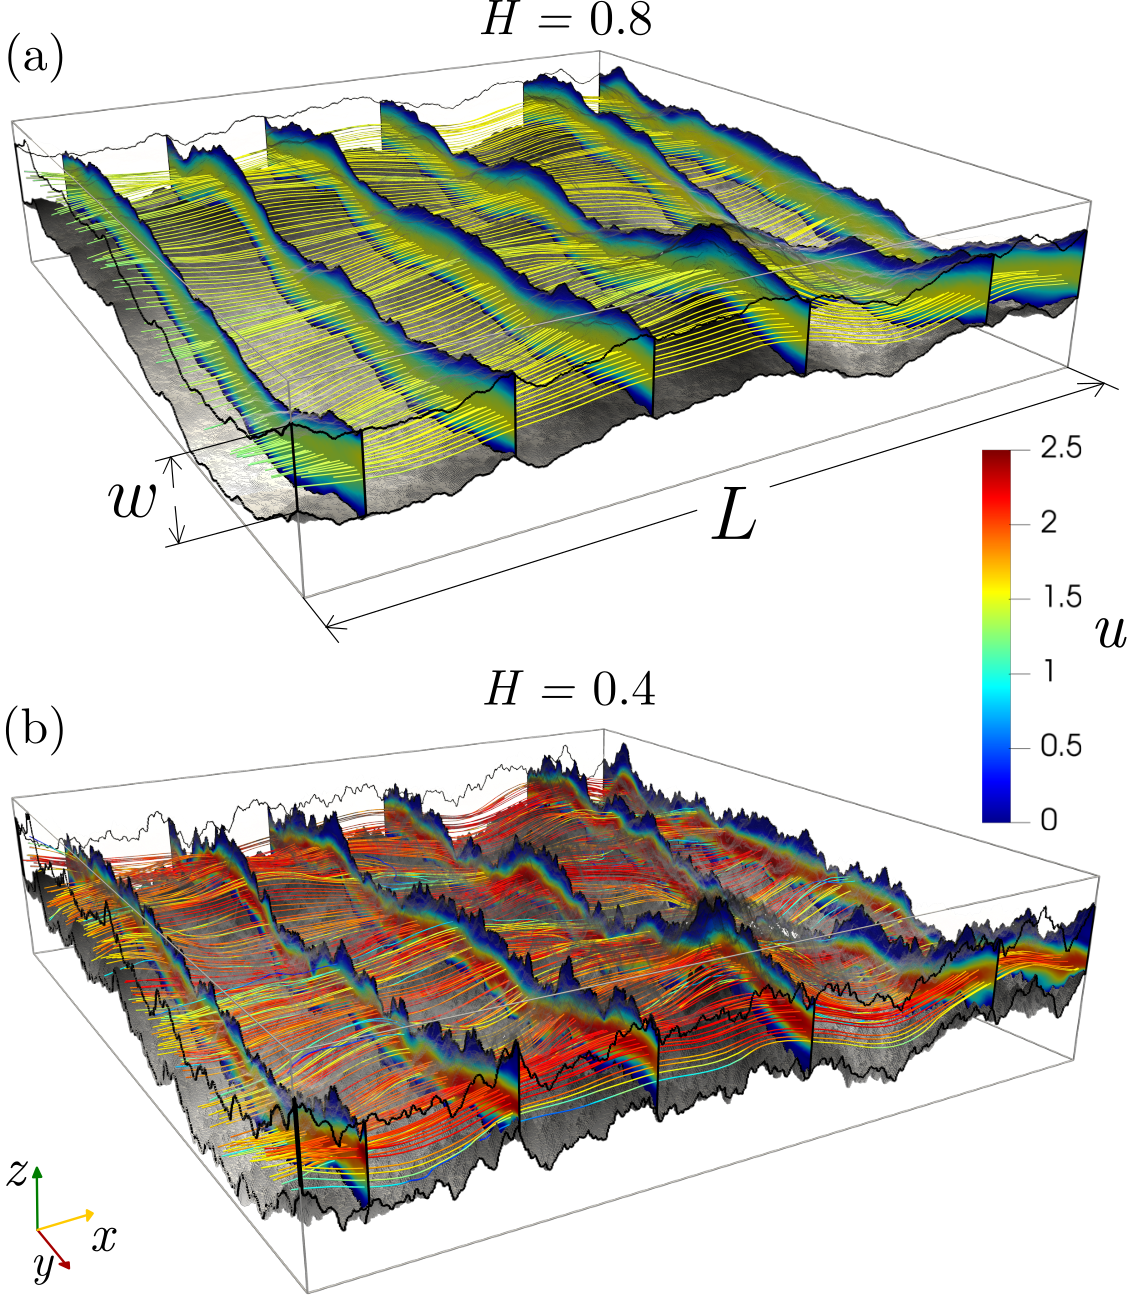
\includegraphics[width=1.00\columnwidth]{fig1.png} %
	\caption{Fluid flow through a typical fracture joint calculated for
	$\mathrm{Re}=100$ and Hurst exponents (a) $H=0.8$ and (b) $H=0.4$. The fluid
	flows from left to right. The contour plots correspond to the velocity
	magnitude at different cross sections. Streamlines are also shown, colored
	according to the local velocity magnitude.} \label{fig1}
\end{figure}
%------------------------------------------------------------

The three-dimensional flow through the self-affine fractures is described by the
incompressible Navier-Stokes equations under isothermal steady-state conditions.
Consequently, the momentum and mass conservation equations are read as
%
\begin{gather} 
\rho~\mathbf{u\cdot\nabla u} = -\mathbf{\nabla} p +
\mu~\mathbf{ \nabla }^{2} \mathbf{u}~, \label{Eq_momentum} \\
{\bf{\nabla\cdot u}}=0~, \label{Eq_continuity}
\end{gather} %
where {\bf u}, $p$ and  $\rho$ are the velocity, pressure, and the fluid's
density, respectively. As boundary condition, we apply non-slip conditions at
the top and bottom walls. Fluid is injected in the $x$ direction at $x=0$ using
a uniform velocity profile with amplitude $U$ at the inlet, and a constant
pressure defines the outlet boundary, at $x=L$. Laterally symmetrical boundary
conditions were applied to minimize finite-size effects. In order to solve
Eqs.~(\ref{Eq_momentum}) and~(\ref{Eq_continuity}) numerically, we first
discretize the volume between the top and bottom surface of the crack using a
tree-dimensional unstructured hexahedral mesh generated by the OpenFOAM's
meshing tool \emph{snappyHexMesh}~\cite{OF_Weller1998}. Close to the surface,
the hexahedral cells were refined three times in order to capture small
variations of the fracture surface over several orders of magnitude.

For different values of the Hurst exponent in the range $0.3 \le H \le 0.9$, we
generated five realizations of the computational domain to compute ensemble
averages. This results in a total of $7\times 5=35$ computational domains. We
then, for each realization, systematically vary the Reynolds number from
$\mathrm{Re}=0.01$ up to $\mathrm{Re}=500$ by adjusting the inlet velocity $U$.

% Results and discussion ----------------------------------------
\section{Results and Discussion}\label{sec:results}

The Forchheimer equation~\cite{Forchheimer1901, Whitaker1996} has been widely
used to describe inertial corrections to Darcy's law for the bulk flow through
disordered pore structures~\cite{Sahimi2000,Sahimi2011,Dullien1992}. Up to cubic
order these corrections can be written as,
%
\begin{equation} 
-\frac{\Delta P}{L} = \alpha \mu U + \beta \rho {U^2} + \frac{\gamma \rho^{2}
	U^{3}}{\mu}~, 
\label{Eq_cubic} 
\end{equation}
%
where $\alpha$ corresponds to the reciprocal of the permeability of the
channel, and $\beta$  and $\gamma$  are the coefficients of the second- and
third-order corrections, respectively. Empirical evidence indicates that
the addition of third-order corrections in the velocity to the Forchheimer
equation allows for an excellent agreement with experimental data for the
full range of the laminar regime ~\cite{Sahimi1994, Edwards1990,
	Andrade1999, Hill2001}. Here  we adopt this approach to characterize the
effect of the convective influence on the flow through the self-affine
channel. 

Rewriting Eq.\eqref{Eq_cubic} in terms of $\mathrm{Re}$, we obtain,
%
\begin{equation} 
G = \alpha w^2 + \beta w \mathrm{Re} + \gamma \mathrm{Re}^{2},
\label{Eq_conductance} 
\end{equation} 
%
where $G \equiv -\Delta P w^{2}/ \mu U L$ is a dimensionless measure of the
{\it hydraulic resistance}. Figure~\ref{fig2} displays the results from
$t\times5\times20=700$ numerical simulations, where $G$ is plotted as a function
of Reynolds number. For each value of the parameters $\mathrm{Re}$ and $H$,
the value of $G$ is obtained as the average over a total of five
realizations. Using the ensemble averages of $G$, we then fit
Eq.~\eqref{Eq_conductance} to the data in order to determine the
coefficients  $\alpha$, $\beta$ and $\gamma$.  

%------------------------------------------------------------
\begin{figure}[!h] 
	\centering 
	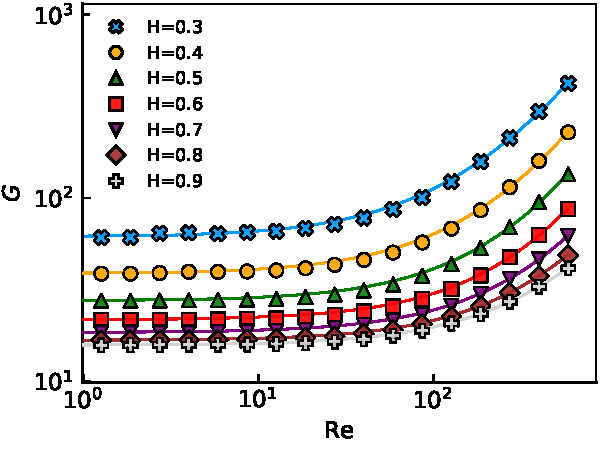
\includegraphics[width=0.99\columnwidth]{fig2.pdf} %
	\caption{ Dependence of the hydraulic resistance $G$ on the Reynolds number
		$\mathrm{Re}$ for different values of the Hurst exponent $H$. In all cases,
		the
		plateau corresponding to Darcy's law (constant $G$) is followed by a
		non-linear
		regime that reflects the effect of convection on the flow. The error bars are
		smaller than the symbols and the solid lines are the best fit to the data
		using
		Eq.~\eqref{Eq_conductance}.} \label{fig2} \end{figure}
%------------------------------------------------------------

For small Reynolds numbers, $G$ is dominated by the first term in
Eq.~\ref{Eq_conductance}, namely $\alpha w^2$. This quantity decreases
monotonically with the Hurst exponent $H$ as shown in the inset of
Fig.~\ref{fig3}, approaching the limiting value $\alpha = 12/w^2$, for a
fracture constituted  of two parallel planes with constant aperture $w$, as
$H$ tends to one.

In order to understand the particular form of this dependence we consider
the fracture as composed of a sequence of parallel plates with varying
angles with respect to the x-y plane. For this very simplified model the
quantity the inverse of the permeability can be approximated by the 
expression
\begin{equation}\label{eq_alphaw2}
\alpha w^2 \propto \tau
\end{equation}
where $\tau \equiv L_p/L$, with $L_p$ being the perimeter of the fracture
in the direction of the flow. In this way, $\tau$ represents the tortuosity
of the fracture. For a self-affine fracture surface one finds
\begin{equation}\label{eq_tau}
\tau = \sqrt{1+\frac{\sigma_z^2}{\delta x^2} \left( \frac{\delta
		x}{L}\right)^{2H}}
\end{equation}
where $\delta x$ is the resolution used to compute the perimeter $L_p$.

Figure~\ref{fig3} shows the $\alpha w^2$ follows very closely
Eq.~\eqref{eq_alphaw2} for small values of $H$.  The solid line represents a fit
to the data combining Eqs.~\eqref{eq_alphaw2} and ~\eqref{eq_tau} with
$\sigma=5$ and $\delta x = 2$. The fit corresponds to $\alpha w^2 = a+b \tau$
with $a=-42.4\pm0.7$ and $b=58.9\pm0.6$ with a Person's $R^2=0.97$. For larger values of the Hurst exponent
($H> 0.7$) the tortuosity of the fluid flow is smaller than the tortuosity of
the surface due to dynamical effects even for very low Reynolds numbers, and the
simplified model described above is expected to overestimate $\alpha w^2$.

%------------------------------------------------------------

\begin{figure} %
	\centering %
	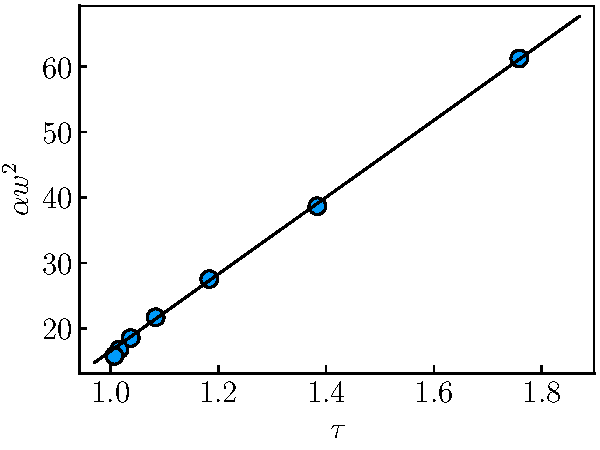
\includegraphics[width=0.99\columnwidth]{fig3.pdf} \caption{Variation of
		$\alpha w^2$ with the tortuosity $\tau$. The error bars are smaller than the
		symbols sizes. The inset shows the dependence of $\alpha w^2$ with the Hurst
		exponent $H$. The solid lines correspond to the least-squares fit using
		$\alpha
		w^2=a + b \tau$, with $a=-42.4\pm0.7$ and $b=58.9\pm0.6$, where $\tau$ was
		computed with $\sigma_z=5$ and $\delta = 2$.}\label{fig3} %
\end{figure}

In agreement with experiments~\cite{Chen2017a}, we observe that the transition
from a linear (constant $G$) to a non-linear regime occurs at lower
$\mathrm{Re}$ for increasing surface roughness. Although the absolute value of 
$G$ significantly depends on the tortuosity, and decreases with $H$, the general
increasing trend of the nonlinear corrections as a funcion of $\mathrm{Re}$
seems to be independent of the Hurst exponent.

In order to quantify the impact of the surface roughness on the departure from
Darcy's law, we plot $G$  as a function of $ \mathrm{Re}/H $. Following this
procedure, all hydraulic conductivity curves collapse onto a single master
curve, as shown in Fig.~\ref{fig4}. This collapse is an indication that the
onset of the non-linear contributions to the hydraulic resistance decreases in a
linear fashion with the tortuosity parameter $\tau$. As a matter of fact, the
excellent quality of the collapse implies the scaling relations $ \beta w
\propto \alpha w^2/H $ and $ \gamma \propto \alpha w^2/H^2 $. As depicted in
Fig.~\ref{fig5}, the second-order term follows the proposed scaling
relations rather well. For the third-order coefficient, however, we observe significant deviations
from the proposed linear trend for $H<0.4$ ($\alpha w^2/H^2 > 110$).
%------------------------------------------------------------
\begin{figure} [!h] %
	\centering %
	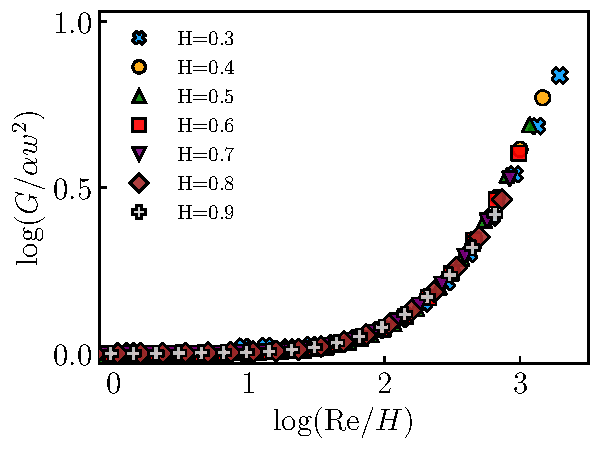
\includegraphics[width=0.99\columnwidth]{fig4.pdf} \caption{Hydraulic
		resistance
		$G$ as a function of $\mathrm{Re}/H$. The excellent collapse of the
		simulation
		data onto a single curve is an indication that the onset of the nonlinear
		contributions to the hydraulic resistance increases approximately linearly
		with
		the Hurst exponent.} \label{fig4} %
\end{figure} %------------------------------------------------------------

%------------------------------------------------------------    
\begin{figure}[!h] %
	\centering %
	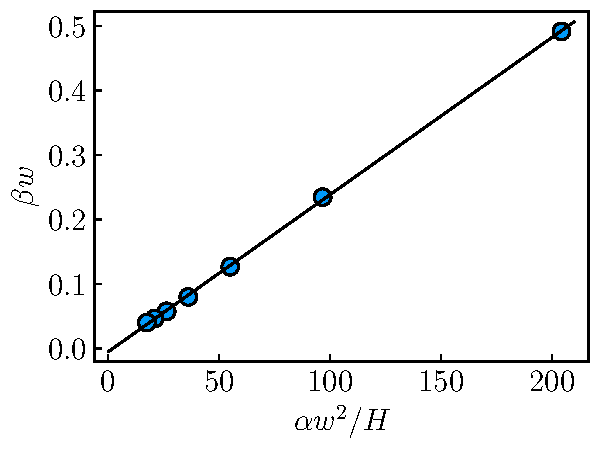
\includegraphics[width=0.99\columnwidth]{fig5.pdf} 
	\caption{(a) The parameter $\beta w$ as a function of $ \alpha w^2/H$. 
		The solid line corresponds to the least-squares fit to the data using 
		$\beta w = c_0 \left(\alpha w^2/H\right) $ with $ c_0=0.0023 \pm 0.0001$. 
		The resulting Pearson coefficients is $ R^2 = 0.9997 $. The inset shows the scaling of
		$\gamma$ with $\alpha w^2/H^2$. The dashed line corresponds to $ \gamma = c_1
		\left(\alpha w^2/H^2\right) + c_2$ with $c_1 = (-1.01\pm0.05)\times10^{-6}$
		and $c_2 = (-1.03\pm0.1)\times10^{-6}$. The simulation data deviates from the
		expected linearity for small $H<0.4$ ($\alpha w^2/H^2 > 110$).} 
	\label{fig5} %
\end{figure}
%------------------------------------------------------------

Next, we analyze the impact of the surface roughness on the velocity field directly. 
Figures~\ref{fig1}a and b show typical realizations
of fluid flows through fracture joints at $\mathrm{Re} = 100$ for Hurst
exponents $H = 0.4$ and $H = 0.8$, respectively. The contour plots show the
magnitude of the velocity field in different cross sections perpendicular
to the main flow direction and streamlines of the velocity field are 
colored by the velocity magnitude. For the larger Hurst exponent, $H =
0.8$, the fluctuations in the local velocity field are visually smoother,
with the maximum velocity near the center of the channel approximately
equal to $3U/2$, as expected for parallel plates. For $H=0.4$, however, the
situation is rather different. Due to continuity, regions of higher
velocities are clearly more confined at the center of the channel, since the
zones of almost stagnated flow close to walls broadens. As a
consequence, the maximum velocity magnitude approaches $5U/2$, effectively
increasing the Reynolds number, as suggested by the collapse in
Fig.~\ref{fig4}. An enhancement in the velocity magnitude due to local
disorder in the surface morphology can then persist and propagate further
into the fracture joint forming preferential flow paths, where the fluid
follows trajectories connecting ``valleys'' and around ``mountains'' of the
rough surfaces. This effect is only possible in three-dimensional flows,
since in two dimensions the flow is forced through local bottlenecks. 

A similar channelization effect has been found in previous
experiments~\cite{Ishibashi2015} and computational simulations~\cite{Drazer2002,
	Lo2014, Huang2017}. This effect, however, was always associated to an additional
shear displacement between the upper and lower surface, which generates a
heterogeneous aperture distribution throughout those fractures.
Our simulations, however, show that no lateral displacement is needed and that
the channelization effect thus must a result of an effective aperture field
which is significantly affected by surface topology.

The  effect of channelization can be quantified by the participation ratio
$\pi$, which describes the spatial localization of kinetic energy inside
the flow~\cite{Andrade1999}. The participation ratio is defined as
\begin{equation}
\pi = \frac{\left<e\right>^2}{\left<e^2\right>},
\end{equation}
where $ \left<e^n\right> = (1/V) \iiint
\left(\mathbf{u}\cdot\mathbf{u}\right)^{n} \; d^3\mathbf{r} $ is the $
n^{th} $ moment of the kinetic energy and $ V $ is the volume of the
system. If the kinetic energy is uniformly distributed across the sample,
one obtains $\pi \rightarrow 1$, whereas if the flow field is strongly
localized, $ \pi \rightarrow 1/V$, approaching zero in the limit of a
infinitely large system. 

Figure~\ref{fig6} shows the variation of  $\pi$ as a function of $H$ for
$\mathrm{Re} = 100$, where the results are obtained by statistically
averaging over five realizations. For $H\rightarrow 1$ the normalized Hurst
exponent approaches a value of $\pi_0=0.7$ which is the expected value for
a Poiseuille flow between two parallel plates. By decreasing $H$, the
participation ratio decreases monotonically indicating a stronger
preferential channeling effect. Also shown in Fig.~\ref{fig6}  is the
participation ratio computed only in the  $ w/2 $-iso distance, defined by
the vertical half distance between the lower and upper boundary of the
crack. Compared to the bulk flow, the kinetic energy is mostly
homogeneously distributed in this surface as the effect fo the wall
roughness is minimal. In this case, $\pi$ also increases with the Hurst
exponent, reflecting the formation of flow channels in fractures generated
with low values of $H$.

\begin{figure}%
	\centering %
	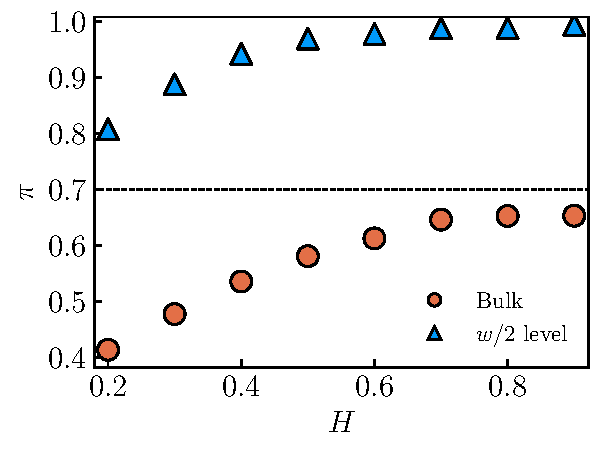
\includegraphics[width=0.99\columnwidth]{fig6.pdf} \caption{Participation
		index
		$\pi$ as a function of the Hurst exponent $H$. Red circles correspond to the
		bulk participation index and the blue squares denote the participation index
		in
		the $w/2$-level surface, obtained by translating the bottom surface of the
		channel by $w/2$ in the $ z $-direction. The dashed horizontal line
		corresponds
		to $\pi=\pi_{0}$, the value of participation for the flow at low
		$\mathrm{Re}$
		between two parallel plates.} \label{fig6} %
\end{figure}


\section{Conclusions}\label{conclusion}

In summary, we have presented an intensive numerical study of single-phase flow in
self-affine fracture joints. We find that each of the coefficients $\alpha$,
$\beta$ and $\gamma$, characterizing the cubic generalization of the Darcy's
equation (\ref{Eq_cubic}) increase exponentially with $H^{-1}$. Our results
indicate that, in the range of Reynolds number  we investigated, these
coefficients are not all independent. Moreover,  inertial effects on the
overall flow can be understood in terms of a universal curve (independent of
$H$) relating the fracture hydraulic conductance and Reynolds number. We
also find that preferred flow paths arise in the flow field, indicating
that, even in three-dimensional fracture joints with no shear displacement
between top and bottom surfaces, the effective fracture aperture field is
heterogeneous.


\begin{acknowledgments}
	We thank the Brazilian agencies CNPq, CAPES and FUNCAP, also the National
	Institute of Science and Technology for Complex Systems and Petrobras for
	financial support. 
\end{acknowledgments}

\bibliography{references}    
\end{document}

